\chapter {Element Attributes}
\label{c:attrib}

%-----------------------------------------------------------------
\section{Dependent and Independent Attributes} 
\label{s:depend} 

For convenience, \bmad\ computes the values of some attributes based
upon the values of other attributes. These dependent variables are
listed in Table~\ref{t:dependent}. Also shown in
Table~\ref{t:dependent} are the independent variables they are
calculated from.  In the table \vn{n_part} and \vn{l_lattice} (lattice
length) are lattice attributes, not element attributes. The first two
are set by the \vn{parameter} statement (See
Section~\ref{s:parameter}). \vn{l_lattice} is calculated when the
lattice is read in.

\begin{table}[h]
\centering {
\begin{tabular}{|l|l|l|} \hline
{\em Element}  & {\em Dependent Variables}  & {\em Independent Variables}  \\ \hline
  BeamBeam     & bbi\_const           & 
                               charge, sig\_x, sig\_y, beam\_energy, n\_part  \\ \hline
  ElSeparator  & e\_field, voltage    & hkick, vkick, gap, l, beam\_energy    \\ \hline
  LCavity      & e\_loss, delta\_e    & gradient, l                           \\ \hline
  RBend, SBend & rho, angle, l\_chord & g, l                                  \\ \hline
  Wiggler (periodic type)
               & k1, rho              & b\_max, beam\_energy                  \\ \hline
\end{tabular}
}
\caption[Table of dependent variables.]{Table of dependent variables and 
  the independent variables 
they are calculated from.}
\label{t:dependent}
\end{table}

No attempt should be made to set or vary within a program dependent
attributes. It should be remarked that this is not an iron clad rule.
If a program properly bypasses \bmad's attribute bookkeeping routine
then anything is possible. In a primary lattice file \bmad\ allows the
setting of a select group of dependent variables if the appropriate
independent is left unspecified.  The list of settable dependent
variables is given in Table~\ref{t:dep_except}.  After reading in the
lattice \bmad\ will set the appropriate independent variable based
upon the value of the dependent variable. \vn{harmon} is the exception in 
that it will never be set by the bookkeeping routine.
\begin{table}[h]
\centering {
\begin{tabular}{|l|l|l|} \hline
{\em Element}  & {\em Dependent Variable Set}  & {\em Independent Variables Not Set}  \\ \hline
  LCavity      & delta\_e                  & gradient                           \\ \hline
  RBend, SBend & rho                       & g                                  \\ \hline
  RBend, SBend & angle                     & g                                  \\ \hline
  RFcavity     & rf\_frequency             & harmon                             \\ \hline
\end{tabular}
}
\caption {Dependent variables that can be set in a primary lattice file.}
\label{t:dep_except}
\end{table}




The normal attribute used to vary the strength of, say, a
\vn{quadrupole} is \vn{k1}.  It is sometimes convenient to be able to
vary the magnetic field strength directly instead. To do this \bmad\ has
a rule that if the appropriate field attribute appears with non-zero value in the
primary lattice file then it becomes a dependent variable and the strength attribute
becomes a dependent variable as tabulated in Table~\ref{t:dep_field}.
\begin{table}[h]
\centering {
\begin{tabular}{|l|l|l|} \hline
  {\em Element} & {\em Strength Attribute} & {\em Field Attribute} \\ \hline
  SBend         &   g                      &  b\_field        \\ \hline
  Solenoid      &   ks                     &  b\_field        \\ \hline
  Quadrupole    &   k1                     &  b\_gradient     \\ \hline
  Sextupole     &   k2                     &  b\_gradient     \\ \hline
  Octupole      &   k3                     &  b\_gradient     \\ \hline
\end{tabular}
}
\caption {Field and Strength Attributes.}
\label{t:dep_field}
\end{table}

%-----------------------------------------------------------------
\section{Type, Alias and Descrip Attributes}
\label{s:string}

\vn{type}, \vn{alias}, and \vn{descrip} are labels to be attached 
to an element. \bmad\ routines do not use these labels except 
when printing element information. \vn{type}
and \vn{Alias} can be up to 16 characters in length and \vn{descrip}
can be up to 200 characters. The attribute strings can be enclosed in
double quotation marks ("). The attribute strings may contain
blanks. If the attribute string does not contain a blank then the
quotation marks may be omitted. In this case the first comma (,) or
the end of the line marks the end of the string. Example:
\begin{example}
  Q00W: Quad, type = "My Type", alias = Who_knows, &
                                  descrip = "Only the shadow knows"
\end{example}

%-----------------------------------------------------------------
\section{Offset, Pitch, Tilt, and Roll Attributes}
\label{s:offset}

There are up to 7 attributes that can offset a physical element
from the reference orbit. They are
\begin{example}
  x\_offset
  y\_offset
  s\_offset
  x\_pitch
  y\_pitch
  tilt
  roll
\end{example}
The exception here is the \vn{pitch} element which uses these
attributes to modify the reference orbit itself.

\vn{x_offset} translates an element in the local $x$--direction
as shown in Figure~\ref{f:pitch}. Similarly, \vn{y_offset} and 
\vn{s_offset} translate an element along the local $y$ and 
$z$--directions respectively. For a bend it is assumed that
the bend angle is small and the rotation of the local reference
axes through the bend is ignored.

The \vn{x_pitch} attribute rotates an element about the $y$--axis
so that the exit face of the element is displaced in the 
$+x$--direction as shown in figure~\ref{f:pitch}. Similarly
the \vn{y_pitch} attribute rotates an element about the $x$--axis
so that the exit face of the element is displaced in the 
$+y$--direction. The rotations
are about the center of the element which is in contrast to the 
\vn{dtheta} and \vn{dphi} misalignments of \mad\ which rotate
around the entrance point. In terms of rotation angle
\begin{example}
  x_pitch =  dtheta
  y_pitch = -dphi
\end{example}
In both \bmad\ and \mad\ offsets are applied before pitches.
\begin{figure}
  \centering
  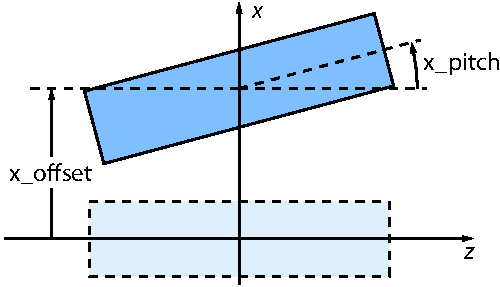
\includegraphics{pitch.psfig}
  \caption{Geometry of Pitch and Offset attributes}
  \label{f:pitch}
\end{figure}

\begin{figure}
  \centering
  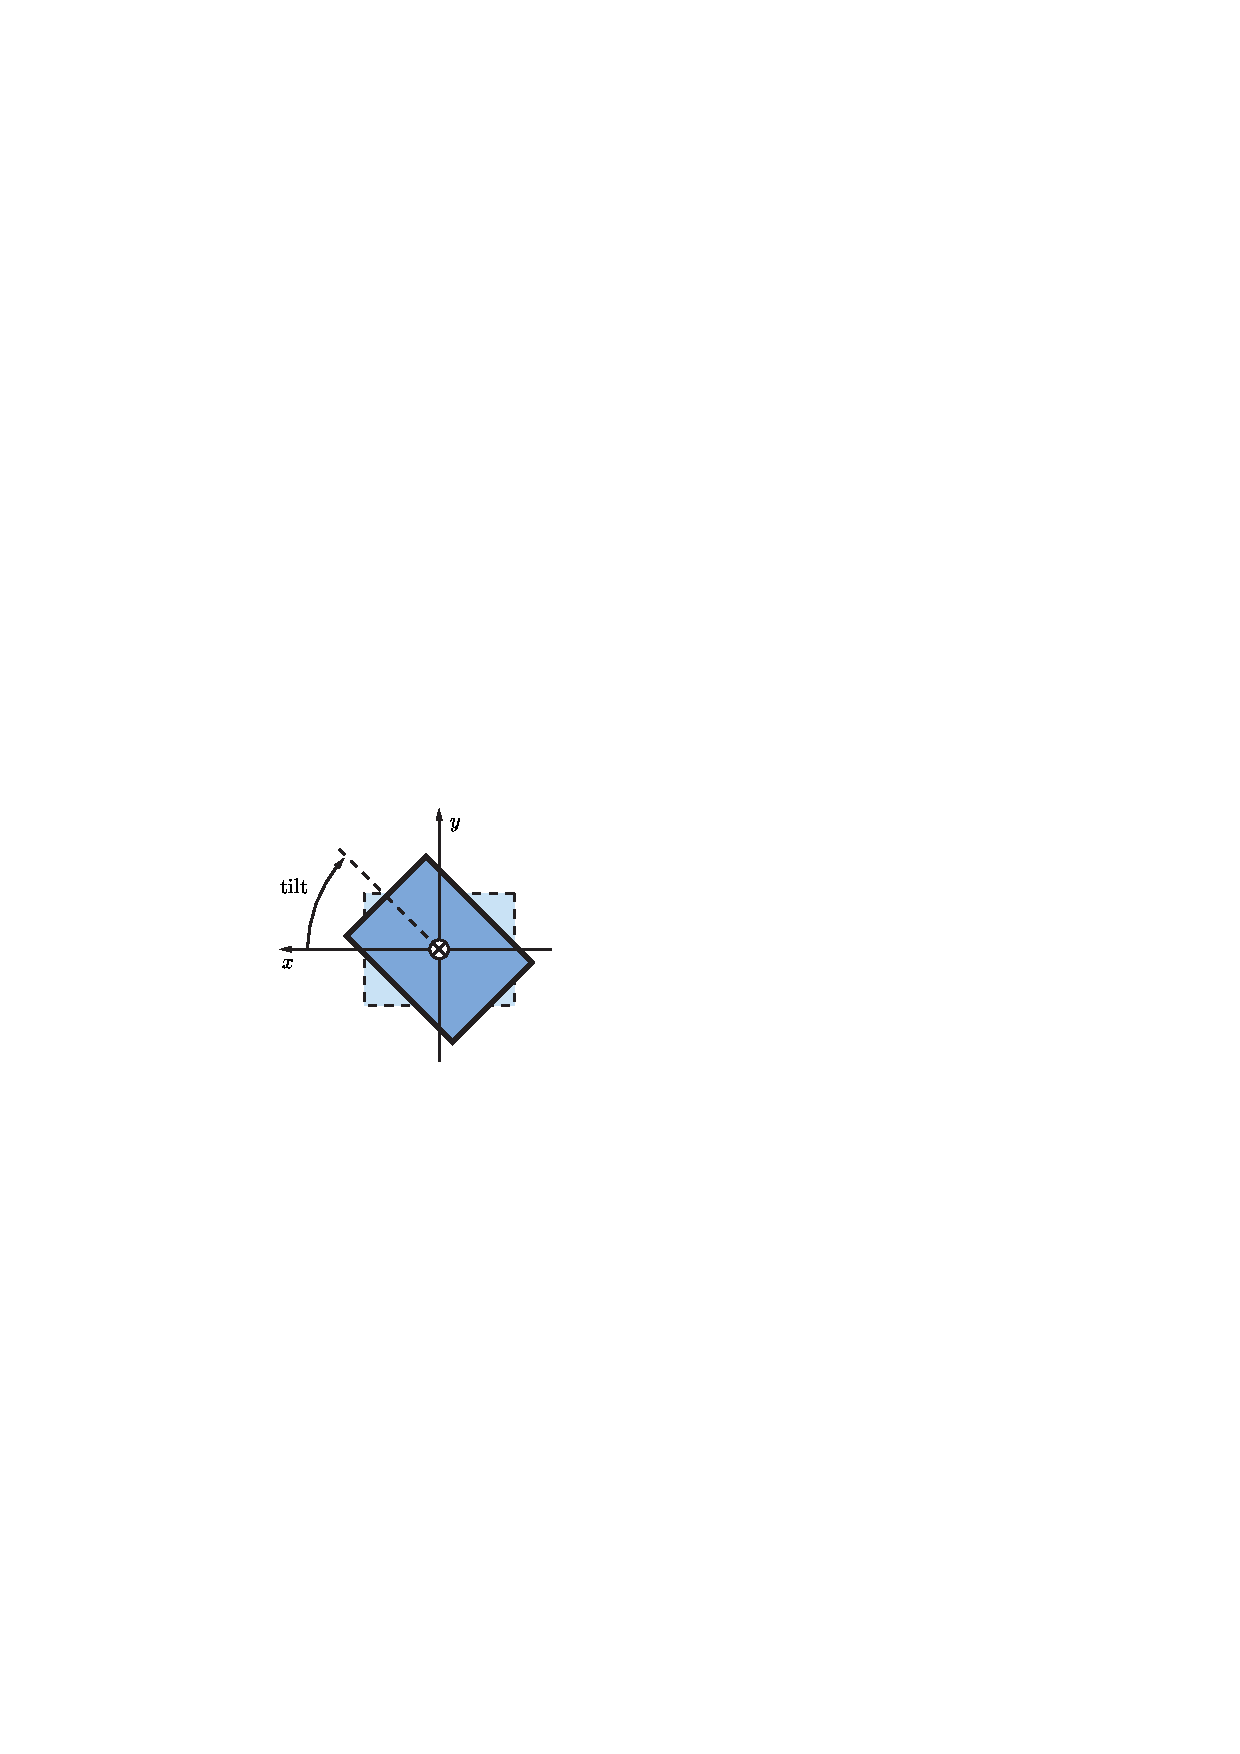
\includegraphics{tilt.psfig}
  \caption{Geometry of a Tilt}
  \label{f:tilt}
\end{figure}

The tilt attribute rotates the element in the $(x, y)$ plane as
shown in figure~\ref{f:tilt}. For a bend the rotation axis is the
$z$-axis at the entrance face. The reference orbit is also rotated
with the element. A bend with a tilt of $\pi/2$ will bend a beam
upward vertically. The \vn{hkick} and \vn{vkick} attributes are
not affected by \vn{tilt} except for \vn{Kicker} and \vn{ElSeparator}
elements
Like MAD, \bmad\ allows the use of the \vn{tilt} attribute without
a value to designate a skew element. For example
\begin{example}
  q1: quad, l = 0.6, x_offset = 0.03, y_pitch = 0.001, tilt
\end{example}
Default tilts can be used for \vn{rbend}, \vn{sbend}, \vn{sol_quad},
\vn{quadrupole}, \vn{sextupole}, and \vn{octupole} elements.
The default tilt is $\pi/n$ where $n$ is the number of poles of the
element (bends have 2, quadrupoles have 4, etc.) 


The \vn{roll} attribute is only used for bends
and rotates the bend, along an axis that runs through the entrance
point and exit point as shown in figure~\ref{f:roll}. A \vn{roll} 
does not affect the reference orbit. The major effect of a \vn{roll}
is to give a vertical kick to the beam.
\begin{figure}
  \centering
  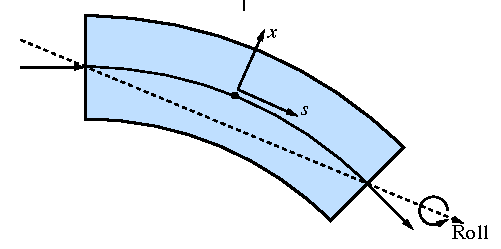
\includegraphics{roll.psfig}
  \caption{Geometry of a Roll}
  \label{f:roll}
\end{figure}


%-----------------------------------------------------------------
\section{Hkick, Vkick, and Kick Attributes}
\label{s:kick}

\vn{kick}, \vn{hkick}, and \vn{vkick} attributes are the integrated
kick of an element in radians. \vn{kick} is only used for \vn{Hkicker}
and \vn{Vkicker} elements. All other elements that can kick use 
\vn{hkick} and \vn{vkick}. The \vn{tilt} attribute will only rotate
a kick for \vn{Hkicker}, \vn{Vkicker}, \vn{ElSeparator} and \vn{Kicker}
elements. This rule was implemented so that, for example, the 
\vn{hkick} attribute for a skew quadrupole
would represent a horizontal steering.

%-----------------------------------------------------------------
\section{Aperture and Limit Attributes}
\label{s:limit}

\begin{figure}
  \centering
  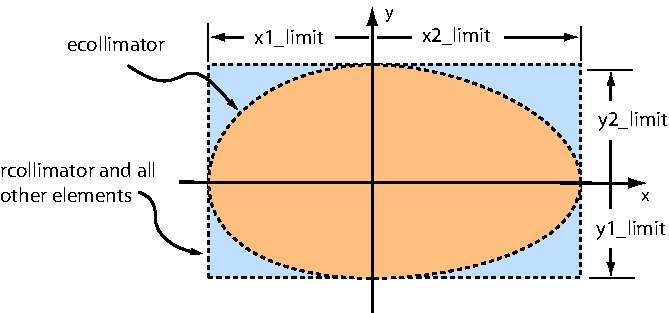
\includegraphics{apertures.psfig}
  \caption{Apertures for ecollimator and rcollimator elements}
  \label{f:limit}
\end{figure}

\vn{x_limit}, \vn{y_limit} specify the half--width of the 
aperture of an element as shown in figure~\ref{f:limit}. 
The aperture is evaluated at the exit
face only of the element. A zero \vn{x_limit} or \vn{y_limit}
is interpreted as no aperture in the $x$ or $y$ direction.
\vn{x_offset} and \vn{y_offset} move the aperture but not pitches or tilts.

An \vn{aperture} attribute supersedes
any \vn{x_limit} and \vn{y_limit} values and sets \vn{x_limit} and
\vn{y_limit} equal to the value of \vn{aperture}.

\noindent
Example:
\begin{example}
  q1: quad, l = 0.6
  q1[x_limit] = 0.03
  q1[y_limit] = 0.03
  q1[aperture] = 0.03  ! equivalent to the proceeding 2 lines.  
\end{example}

%-----------------------------------------------------------------
\section{Transfer Maps via Integration}
\label{s:integ}

One way to create a transfer map through an element is to divide the
element up into slices and then to propagate the transfer
map slice by slice.
There are several ways to do this integration. The Boris and Runge--Kutta 
methods integrate the equations of motion to give the 0\Th\ order
transfer map which is just the particle orbit.
Symplectic integration using Lie algebraic techniques, on the other hand, 
can generate maps to any order.
The \vn{num_steps} attribute determines the number of slices. This is
applicable to \vn{Boris}, \vn{Symp_Lie_Bmad}, and \vn{Symp_Lie_PTC}
integration. 

\vn{integration_ord} is the order of the integration formula for 
\vn{Symp_Lie_PTC}. Possible values are
\begin{example}
  integration\_ord = 2 (default), 4, or 6
\end{example}
Essentially, an integration order of $n$ means that the error in an 
integration step scales as $dz^{n+1}$ where $dz$ is the slice thickness.
For a given number of steps a higher order will give more accurate results
but a higher order integrator will take more time per step. It turns out
that for wigglers, after adjusting \vn{num_steps} for a given accuracy, 
the order 2 integrator is the fastest. This is not surprising given the
highly nonlinear nature of a wiggler. Note that \vn{Symp_Lie_Bmad} always
uses a order 2 integrator.

\vn{Adaptive_Boris} and \vn{Runge_Kutta} use adaptive step
control independent of \vn{num_steps}. These methods use the \vn{rel_tol} and
\vn{abs_tol} attributes to try to keep the estimated error of the integration
such that
\begin{example}
  error < abs\_tol + |orbit| * rel_tol
\end{example}
lowering the error bounds makes for greater accuracy (as long as round-off 
doesn't hurt) but for slower tracking. 

\vn{Boris}, \vn{Adaptive_Boris}, and \vn{Runge_Kutta} tracking all use
as input the electric and magnetic fields of an element. 

%-----------------------------------------------------------------
\section{Length Attributes}
\label{s:l}

\vn{l} is, for all elements except \vn{RBend}s, the path length 
of the reference particle.
Note that for wigglers this is not the same as the path length for
a particle with the reference energy starting on the reference orbit.

%-----------------------------------------------------------------
\section{Symplectify Attribute}
\label{s:symp}

A linear transport matrix may be non--symplectic for a number of reasons.
For example, the linear matrix that comes from expanding a Taylor Map
around any point that is not the origin of the map is generally not 
symplectic. The transfer matrix for an element can be symplectified by
setting the \vn{symplectify} attribute to True. See section \ref{s:symp_method}
for details on how a matrix is symplectified. The default value of \vn{symplectify} 
if it is not present is \vn{False}. If it is present without a value then
it defaults to true. Examples:
\begin{example}
  s1: sextupole, l = 0.34                       ! symplectify = False
  s1: sextupole, symplectify = True, l = 0.34   ! symplectify = True
  s1: sextupole, symplectify, l = 0.34          ! symplectify = True
\end{example}

%-----------------------------------------------------------------
\section{Is\_on Attribute}
\label{s:is_on}

The \vn{is_on} attribute is used to turn an element off. Turning
an element off essentially converts it into a drift. This is not
generally used in a lattice file but a program can use the attribute
for, say, calculating the Twiss parameters which needs to be done
with the RF cavities off. Example
\begin{example}
  q1: quad, l = 0.6, k1 = 0.95
  q1[is_on] = False
\end{example}
Note: \vn{is_on} does not affect any apertures that are set.